\section{Data Generation}

Before talking about how to create appropriate models for the detection of
mechanical symbols, it is necessary to gather appropriate data for that task.

The goal is to read handwritten mechanical symbols.
The data to train the model is therefore created by myself and a necessary step in this undertaking.
Since data generation can be time consuming, the data had to be created in a fast pace by allowing to keep the data valid.
Fortunately the author had access to a tablet, which allows to draw directly onto a digital canvas.
To rapidly generate data a few premises for the script had to be considered:
\begin{enumerate}
    \item A drawing context is created.
    \item The context is variable in size and color.
    \item The context should is able to recognize mouse events.
    \item The script should have access to the file system to safe data with no extra work required.
\end{enumerate}

A simple Python script is able to fulfill these demands.
The library \name{OpenCV}\cite{OpenCV2019} allows for the creation of a window with respective attributes. In particular the library \code{opencv-python}\cite{Heinisuo2019} is used as an implementation of \name{OpenCV}.
It fulfills all these requirements, since it allows for the creation of a window with a programmable context and event handlers for mouse interactions\footnote{ The data generation process was considered to be done using JavaScript, but the last requirement to safe data is not as easily fulfilled using packages known to the author as using a python script. Node.js allows to easily safe files but is inherently headless and has therefore no allowance for a context to draw on. }.

Since the model should be able to recognize symbols of arbitrary color on arbitrary background, the context background is a random value in grayscale, as is the line which is drawn on to the background.
The thickness of the line which is used for drawing is also random, imitating the appearance of a smaller symbol (potentially reducing the resolution of the image in a later process).

Having laid out the parameters used for drawing the context is created using
\name{cv2}'s \code{namedWindow} function. For respective interaction the \code{setMouseCallback} function is applied to the \code{namedWindow} created, using a \code{draw} function which allows for mouse events to be recognized and to be acted upon.

Drawing is then done by events respectively named \code{cv2.EVENT\_LBUTTONDOWN} and \code{cv2.EVENT\_LBUTTONUP} which set a boolean \code{drawing} flag to either \code{True} or \code{False}.
Saving the drawn image is done using \code{cv2.Event\_RBUTTONUP}, which names the image after the number of images previously drawn automatically.

The frame for the different classes is set in the beginning of the script, having an interactive command prompt asking the user which class is to be filled next, having the options \textit{"x" for base, "o" for link, "n" for non hits}. The consideration of \textit{non hits} is especially important, since later on on figuring out where on a arbitrary image symbols are to be found, the majority of feedbacks are expected to be no symbol at all.

Using this script 500 symbols for each class are created. These images are expected to be augmented later for a chance to counter overfitting, but for the task of differentiation three different classes they are expected to suffice.

\begin{figure} \label{fig:generated_data_samples}
    \centering
    \begin{subfigure}[b]{0.3\textwidth}
        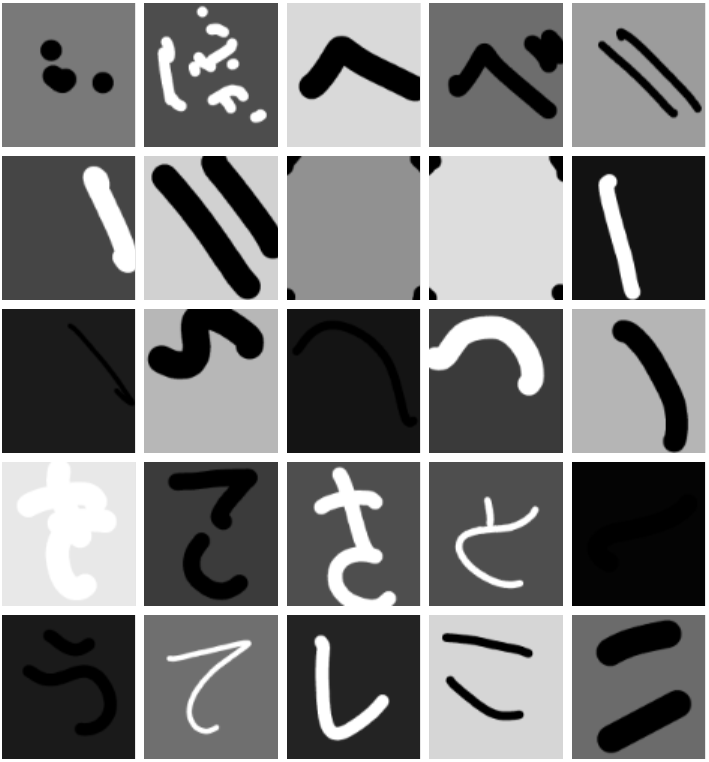
\includegraphics[width=\textwidth]{images/25_n.png}
        \caption{Non hits}
        \label{fig:25_non_hits}
    \end{subfigure}
    \begin{subfigure}[b]{0.3\textwidth}
        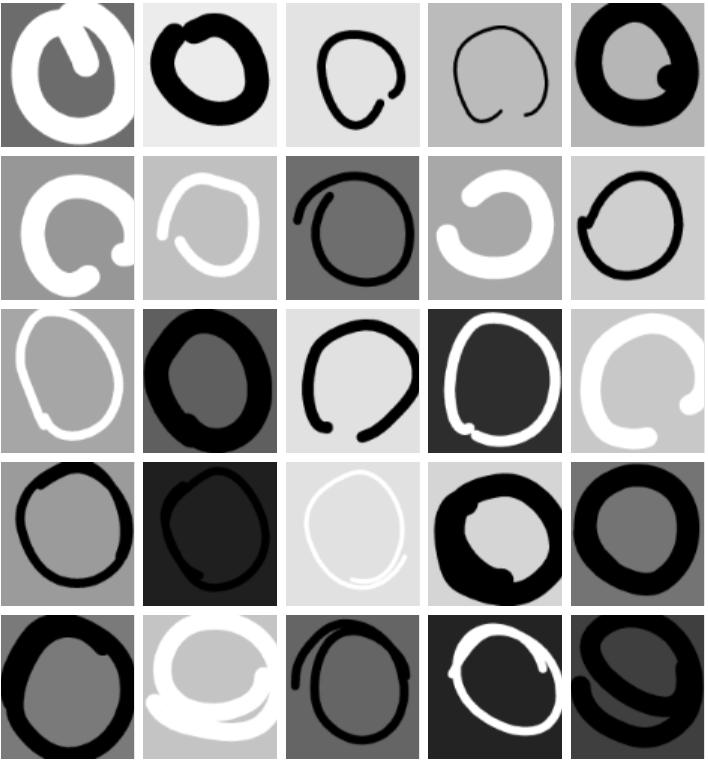
\includegraphics[width=\textwidth]{images/25_o.png}
        \caption{Links}
        \label{fig:25_links}
    \end{subfigure}
    \begin{subfigure}[b]{0.3\textwidth}
        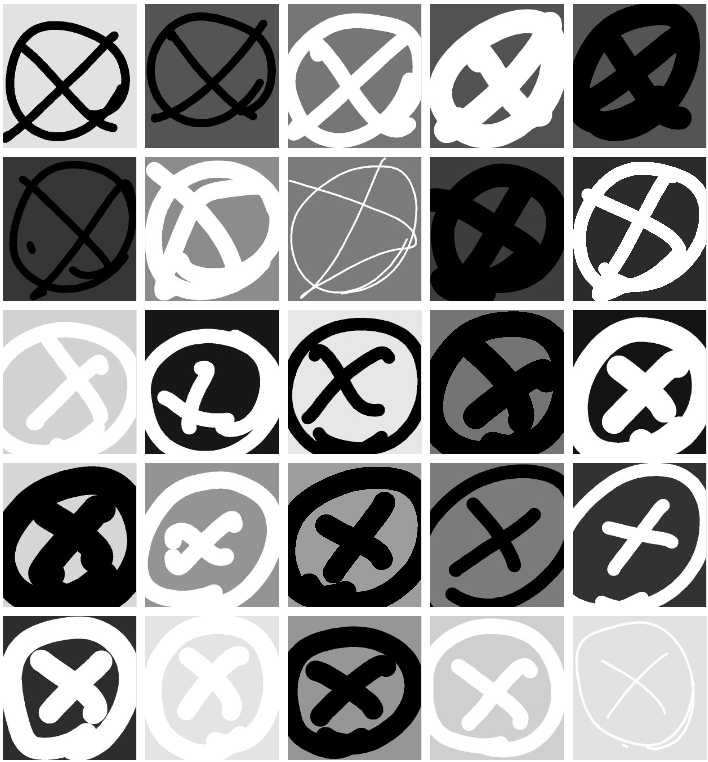
\includegraphics[width=\textwidth]{images/25_x.png}
        \caption{Bases}
        \label{fig:25_bases}
    \end{subfigure}
    \caption{A sample of created data using the described method. For the first tests only these three classes were created. Images are created centered in a square, which is how arbitrary images can be scanned later using squares of different sizes as templates. }
\end{figure}

\footnote{The code can be reviewed at \url{https://klawr.github.io/deepmech/src/data/data_generation.py}} % TODO and in Appendix A?
